\documentclass{scrartcl}

\usepackage{graphicx}
\usepackage[utf8]{inputenc}
\usepackage[T1]{fontenc}
\usepackage{lmodern}
\usepackage{babel}
\usepackage{amsmath}
\usepackage{amsthm}
\usepackage{mathtools}
\usepackage{amssymb}
\usepackage{listings}
\usepackage{xparse}
\usepackage{geometry}
\usepackage{enumerate}
\usepackage{tikz}
\usepackage[style=english]{csquotes}
\usepackage[language=english, backend=biber, style=alphabetic, sorting=nyt]{biblatex}

\usetikzlibrary{babel, positioning, shapes.geometric, arrows, arrows.meta}
\addbibresource{bibliography.bib}

\title{The Supersingular Diffie-Hellmann Key Exchange protocol}
\author{Simon Pohmann}

\newcommand{\N}{\mathbb{N}}
\newcommand{\Z}{\mathbb{Z}}
\newcommand{\F}{\mathbb{F}}
\newcommand{\proj}{\mathrm{proj}}
\newcommand{\Quot}{\mathrm{Quot}}
\renewcommand{\O}{O}

\newtheorem{prop}{Proposition}[section]
\newtheorem{theorem}[prop]{Theorem}
\newtheorem{alg}[prop]{Algorithm}
\newtheorem{definition}[prop]{Definition}
\newtheorem{example}[prop]{Example}
\newtheorem{remark}[prop]{Remark}

\begin{document}

\maketitle

\tableofcontents

\section{Elliptic Curves}

\subsection{The geometric point of view}

\begin{definition}
    A (possibly nonsmooth) elliptic curve $E$ defined over a field $K$ is the (projective) zero set
    \begin{equation*}
        E = \{ (x : y : 1) \ | \ y^2 + a_1 xy + a_3 y = x^3 + a_2 x^2 + a_4 x + a_6 \} \cup \{ \O \} \subseteq \mathbb{P}_{\bar{K}}^2
    \end{equation*}
    of some irreducible polynomial $F(x, y) = y^2 + a_1 xy + a_3 y - x^3 - a_2 x^2 - a_4 x - a_6 \in K[x, y]$. 
    This equation is called a Weierstraß equation defining $E$.
    The point $\O := (0 : 1 : 0)$ here is the point at infinity of the elliptic curve.
\end{definition}

\begin{definition}
    \label{def:discriminant}
    A (possibly nonsmooth) elliptic curve $E$ defined by $y^2 + a_1 xy + a_3 y = x^3 + a_2 x^2 + a_4 x + a_6$ is called smooth, if the discriminant
    \begin{align*}
        \Delta(E) = & - b_2^2 b_8 - 8 b_4^3 - 27 b_6^2 + 9 b_2 b_4 b_6 \\
        \text{where} \ & b_2 = a_1^2 + 4 a_2 \\
        & b_4 = a_1 a_3 + 2 a_4 \\
        & b_6 = a_3^2 + 4 a_6 \\
        & b_8 = a_1^2 a_6 + 4 a_2 a_6 - a_1 a_3 a_4 + a_2 a_3^2 - a_4
    \end{align*}
    is nonzero. In this work, the term ``elliptic curve'' will be used for smooth elliptic curves.
\end{definition}

As elliptic curves are given as the zero set (or locus) of a polynomial, they are algebraic varieties and many properties can be studied using Algebraic Geometry.
In the more general context of Algebraic Geometry, an elliptic curve is usually defined as a smooth projective curve of genus 1.
As shown in \cite[III Prop 3.1]{arithmetic_elliptic_curves}, each elliptic curve by this definition is isomorphic to an elliptic curve defined by a Weierstraß equation.
Here ``isomorphic'' refers to $K$-variety isomorphisms in the sense of Algebraic Geometry.
As this is a fundamental notion, we will state the required special case here.

\begin{definition}
    For a (projective) algebraic variety $V \subseteq \mathbb{P}_{\bar{K}}^2$ given as the zero set of an ideal $I \leq K[x, y, z]$, its (projective) coordinate ring is given as $K^+[V] := K[x, y, z] / I$.
\end{definition}

\begin{definition}
    Given irreducible varieties $V, W \subseteq \mathbb{P}_{\bar{K}}^2$, a partial map $\phi: V \to W$ is called rational if it is given by rational functions.
    Namely, $\phi$ is rational if there are homogeneous $f_1, f_2, f_3 \in \bar{K}^+[V]$ of same degree and not all zero such that for each point $(x : y : z)$ at which $\phi$ is defined, there are ``equivalent'' polynomials $(g_1, g_2, g_3) \in \bar{K}^+[V], \ (g_1, g_2, g_3) \sim (f_1, f_2, f_3)$ such that
    \begin{equation*}
        (g_1(x, y, z) : g_2(x, y, z) : g_3(x, y, z)) \ \text{is nonzero and equal to $\phi(x : y : z)$}
    \end{equation*}
    Here we define equivalence as $(f_1, f_2, f_3) \sim (g_1, g_2, g_3)$ if $f_i g_j = f_j g_i$ for all $i, j$.
    We use the notation $\phi = [f_1, f_2, f_3]$ or $\phi = [f_1^{\mathrm{deh}}, f_2^{\mathrm{deh}}, f_3^{\mathrm{deh}}]$
    \footnote{For a homogeneous polynomial $f \in K[x, y, z]$ the notation $f^{\mathrm{deh}}$ is the dehomogenization $f(x, y, 1)$. Note that $f$ corresponds to $f^{\mathrm{deh}}$ uniquely except for scaling by $z$, but scaling by $z$ does not change the defined rational map.}.
    The rational map is said to be defined over $K$, if $f_1, f_2, f_3 \in K^+[V]$.
\end{definition}

This definition is quite technical, as for well-definedness, we require that no denominator polynomial evaluates to 0 and do not get the projective (non-)point $(0 : 0 : 0)$. 

The intuition is that each component of a rational map is given by a quotient of polynomials.
If we want to evaluate the map at a point where the quotient is not well-defined, then we are allowed to ``fix'' it by dividing out a corresponding polynomial factor from all components.
This dividing out of a corresponding polynomial factor does not change the ratio of two homogeneous components, hence it does not change the projective point.
As $\bar{K}[V]$ is not a UFD, defining this division is not straightforward. 
Instead, we define a tuple of polynomials as equivalent, if the ratio of different components is the same in the coordinate ring.
Now equivalent polynomial tuples can be obtained from each other by some kind of ``abstract'' division.

\begin{definition}
    A rational map between varieties that is defined everywhere is called morphism. If it is bijective and its inverse is a morphism, it is called a variety isomorphism.
\end{definition}

These definitions are the general ones from Algebraic Geometry. In the case of elliptic curves however, some parts are simpler than in the general case.
For example, if the domain is a smooth (elliptic) curve, then each rational map is a morphism (see \cite[II Prop 2.1]{arithmetic_elliptic_curves}).
Furthermore, elliptic curves have only one point at infinity, with the result that we can introduce ``special rules'' for $\O$ and forget about the description of points at infinity that is given by projective geometry.
This is described in the next section.

\subsection{The affine point of view}

Because of many reasons, projective geometry is the ``correct'' way to describe varieties, hence elliptic curves are usually defined as projective curves.
To deal with geometric properties of elliptic curves, we will also use the theory of Algebraic Geometry, which heavily relies on projective geometry.
In such a setting, different points on the curve are indistinguishable. 
However, much of the theory of elliptic curves requires a distinguished point.
By defining this point to be ``the point at infinity'', we will not require the rules for working at infinity.
This is not really an affine setting, as we still (and need) the point at infinity, but working in this setting often feels like an affine one.
It is also the convention that the notation focuses on this point of view (as one can already see from our previous definition, which uses non-homogeneous polynomials and ideals).

\begin{remark}
    A (possibly nonsmooth) elliptic curve $E$ defined over a field $K$ is the affine zero set
    \begin{equation*}
        \{ (x, y) \in \bar{K}^2 \ | \ y^2 + a_1 xy + a_3 y = x^3 + a_2 x^2 + a_4 x + a_6 \} \subseteq \bar{K}^2
    \end{equation*}
    of some irreducible polynomial $F(x, y) = y^2 + a_1 xy + a_3 y - x^3 - a_2 x^2 - a_4 x - a_6 \in K[x, y]$ together with a point at infinity $\O := \infty$. 
\end{remark}

\begin{remark}
    A (possibly nonsmooth) elliptic curve $E$ is called smooth, if its discriminant $\Delta(E)$ (see \ref{def:discriminant}) is nonzero. In this work, the term ``elliptic curve'' will be used for smooth elliptic curves.
\end{remark}

Now we come to rational maps and morphisms. First, we require the affine coordinate ring of an elliptic curve.

\begin{definition}
    The affine coordinate ring of an elliptic curve defined by $F(x, y) := y^2 + a_1 xy + a_3 y - x^3 - a_2 x^2 - a_4 x - a_6 = 0$ is given as $K[E] := K[x, y] / (F(x, y))$.
\end{definition}

Note that we may evaluate elements $f \in K[E]$ at points $(x, y) \in E$, as each representative in the equivalence class will evaluate to the same value at $(x, y)$.

The definition of rational maps is somewhat problematic now, as rational maps in general may map $\O$ to a point ``not at infinity''.
However, by considering only rational maps that map $\O$ to $\O$, we can eliminate this problem.
In fact, as the point at infinity has a special role in the theory of elliptic curves, these are also the maps that are most interesting, and thus deserve a new name.

\begin{definition}
    A morphism between elliptic curves $\phi: E \to E'$ that maps $\phi(\O) = \phi(\O)$ is called isogeny.
\end{definition}

We will also use the term ``isomorphism'' for variety isomorphisms that map $\O$ to $\O$.
Maps that are isomorphisms only in the geometric sense (i.e. bijective morphisms whose inverse is a morphism) will be called variety isomorphisms.
We will rarely use them.

\begin{definition}
    A bijective isogeny whose inverse is also an isogeny is called isomorphism (between elliptic curves).
\end{definition}

Now we can find an ``affine'' characterization:

\begin{remark}
    A non-constant map $\phi: E \to E'$ between elliptic curves is an isogeny, if and only if it fulfills the following condition:
    There are elements $f_1, f_2, g \in \bar{K}[E], g \neq 0$ such that for all points $(x, y) \in \bar{K}^2$, there are $f_1', f_2', g' \in \bar{K}[E], g' \neq 0$ with
    \begin{align*}
        \left(\frac {f_1'} {g'}, \frac {f_2'} {g'}\right) = \left(\frac {f_1} g, \frac {f_2} g\right) \ &\text{in the field of fractions of $K[E]$ and} \\
        \left(\frac {f_1'(x, y)} {g'(x, y)}, \frac {f_2'(x, y)} {g'(x, y)}\right) \ &\text{is defined and equal to $\phi(x, y)$}
    \end{align*}
    Here we say that only $(\frac 0 0, \frac 0 0)$ is not defined, and let $(\frac a 0, \frac b 0) := \O = \infty$ for $(a, b) \neq (0, 0)$.
    We use the notation $\phi = [f_1, f_2, g]$.
\end{remark}

\subsection{A simpler formula}

The general Weierstraß equation is still relatively complicated. If the characteristic of $K$ is not $2$ or $3$ however, we have the following simpler representation:

\begin{prop}
    Let $E$ be an elliptic curve defined over $K$ with $\mathrm{char}(K) \neq 2, 3$ by the Weierstraß equation $y^2 + a_1 xy + a_3 y = x^3 + a_2 x^2 + a_4 x + a_6$.
    Then $E$ is isomorphic to an elliptic curve defined by a Weierstraß equation of the form
    \begin{equation*}
        y^2 = x^3 + Ax + B
    \end{equation*}
    where $A, B \in K$.
\end{prop}
\begin{proof}
    Consider the isogeny given by
    \begin{equation*}
        \phi_1 = \Bigl[ x, y - \frac {a_1 x + a_3} 2, 1 \Bigr]
    \end{equation*}
    Then have that
    \begin{align*}
        &\left( y - \frac {a_1 x + a_3} 2 \right)^2 + (a_1 x + a_3) \left( y - \frac {a_1 x + a_3} 2 \right) \\
        = & \ y^2 - y (a_1 x + a_3) + (a_1 x + a_3) y - \left( \frac {a_1 x + a_3} 2 \right)^2 = y^2 - \frac 1 4 ( a_1 x + a_3 )^2
    \end{align*}
    Let $E_1$ be the elliptic curve defined by 
    \begin{equation*}
        E_1: y^2 = x^3 + \frac 1 4 b_2 x^2 + \frac 1 2 b_4 x + \frac 1 4 b_6
    \end{equation*}
    with $b_2 = 4a_2 + a_1^2$, $b_4 = 2 a_4 + a_1 a_3$ and $b_6 = 4a_6 + a_3^2$.
    Then $\phi_1$ maps $E_1$ to $E$ as by the above computation, $\phi(x : y : z) \in E$ for all $(x : y : z) \in E_1$.
    Furthermore, $\phi_1$ is given by a linear change of coordinates, hence it is an isomorphism.

    Similarly, consider the isogeny given by
    \begin{equation*}
        \phi_2 = \Bigl[ x - \frac {b_2} {12}, y, 1 \Bigr]
    \end{equation*}
    By an analogous computation as above, get that $\phi_2$ is an isomorphism $E_2 \to E_1$ where $E_2: y^2 = x^3 + Ax + B$ for $A = \frac 1 2 (b_4 - \frac 1 {24} b_2^2)$ and $B = \frac 1 4 (\frac 1 6 b_2 b_4 - \frac 1 {216} b_2^3 - b_6)$.
    Composing $\phi_1 \circ \phi_2$ yields an isomorphism between $E_2$ and $E$.
\end{proof}

The reader might compare the $b_2, b_4, b_6$ used in this proof with the definition of the discriminant \ref{def:discriminant} to get an explanation for the choice of some parts of the discriminant formula.
This formula also gets much simpler when using the simplified form.

\begin{remark}
    Let $E$ be an elliptic curve defined by $E: y^2 = x^3 + Ax + B$. Then
    \begin{equation*}
        \Delta(E) = -16(27 B^2 + 4 A^3)
    \end{equation*}
\end{remark}
\begin{proof}
    Just insert $a_4 = A, a_6 = B$ and $a_1 = a_2 = a_3 = 0$ into the definition \ref{def:discriminant}.
\end{proof}

For simplicity, we will from now on assume that the characteristic of $K$ is not $2$ or $3$ and hence use this simpler formula. 
Most proofs work also in the general case, but the involved computations will be more complicated and less instructive.

\subsection{More isomorphisms}

Until now we have seen that each curve is isomorphic to a curve given by a relatively simple equation.
To completely classify whether two curves are isomorphic, it is now left to study when two curves of this form are isomorphic.
This can be done by the so-called j-invariant.

\begin{definition}
    Let $E$ be an elliptic curve defined by $E: y^2 = x^3 + Ax + B$. Then the j-invariant is given by
    \begin{equation*}
        j(E) := \frac {(-48 A)^3} {\Delta(E)} = 1728 \frac {4A^3} {27 B^2 + 4A^3}
    \end{equation*}
\end{definition}

\begin{prop}
    Let $E: y^2 = x^3 = Ax - B$ and $E': y^2 = x^3 - A'x - B'$ be elliptic curves. Then there is an isomorphism $E \to E'$ if and only if $j(E) = j(E')$.
\end{prop}
\begin{proof}
    First, assume $j(E) = j(E')$ and consider the isogeny $\phi = [u^2 x, u^3 y, 1]$ where $u^4 = A/A'$.
    Then
    \begin{align*}
        (u^3 y)^2 =& \ u^6 y^2 \quad \text{and} \\
        (u^2 x)^3 - A (u^2 x) - B =& \ u^6 \Bigl(x^3 - \frac 1 {u^4} A x - \frac 1 {u^6} B \Bigr) \\
        =& \ u^6 \Bigl( x^3 - A' x - \frac 1 {u^6} B \Bigr)
    \end{align*}
    From $j(E) = j(E')$ we get
    \begin{equation*}
        A^3 (27 B'^2 + 4A'^3) = A'^3 (27 B^2 + 4A^3)
    \end{equation*}
    Thus
    \begin{equation*}
        A^3 \left( 27 B'^2 + 4\frac 1 {u^{12}} A^3 \right) = \frac 1 {u^{12}} A^3 (27 B^2 + 4A^3)
    \end{equation*}
    and so
    \begin{equation*}
        B'^2 = \frac 1 {u^{12}} B^2 + \frac 1 {27 u^{12}} (4 A^3 - 4 A^3) = \frac 1 {u^{12}} B^2
    \end{equation*}
    It follows that $u^6 = B/B'$ and so $\phi$ maps $E$ to $E'$. It is only a linear transformation, hence also an isomorphism.

    For the other direction, assume there is an isomorphism $\phi = [x', y', 1]$ from $E$ to $E'$ where $E': y^2 = x^3 + A'x + B'$ and $x', y' \in K[E]$.
    \paragraph{Claim} Then $x = u_1 x' + r$ and $y = u_2 y' + x_2 x' + t$ for $u_1, u_2 \in \bar{K}^*$ and $r, t \in \bar{K}$.
    To prove this claim, we require some advanced Algebraic Geometry. 
    To examine $\O$ using an ``affine'' approach, we change our embedding $K^2 \to \mathbb{P}^2$ such that $(x, z) \mapsto (x : 1 : z)$ and get the affine curve
    \begin{align*}
        E \ &\text{defined by} \ Z = X^3 + A X Z^2 + B Z^3 \ \text{resp.} \\
        E' \ &\text{defined by} \ Z = X^3 + A' X Z^2 + B' Z^3
    \end{align*}
    The curves do not change by this, we just consider another affine part of the projective plane that now contains $\O$. In particular, $\O$ is now the origin $(0, 0)$.
    Note that this is just a conceptual tool, formally this is given by the isomorphism 
    \begin{align*}
        K(E) &= \Quot\left(K[x, y] / (y^2 - x^3 - A x - B)\right) \\
        \cong \ K(\tilde{E}) &= \Quot\left(K[X, Z]/(Z - X^3 - A X Z^2 - B Z^3)\right)
    \end{align*}
    via $x \mapsto X/Z, \ y \mapsto 1/Z$, where $\tilde{E} = E \cap K^2$ is the considered affine part of the curve. 
    We identify those two representations, in particular have $x, y, x', y' \in K(\tilde{E})$.
    
    Now consider the localization
    \begin{equation*}
        R := K[\tilde{E}]_{(0, 0)} := K[\tilde{E}]_{\mathfrak{m}} \subseteq K(\tilde{E}) \ \text{where} \ \mathfrak{m} = \langle x, z \rangle = \{ f \in K[\tilde{E}] \ | \ f(0, 0) = 0 \}
    \end{equation*}
    of the affine coordinate ring $K[\tilde{E}] = K[X, Z]/(Z - X^3 - A X Z^2 - B Z^3)$ at $(0, 0) \in K^2$.
    This is a local ring with unique maximal ideal $\mathfrak{m}$.
    We show that the valuation of $X$ and $X' := x'/y'$ in $R$ is -2.
    Now have that $Z = X^3 + A X Z^2 + B Z^3$ and hence
    \begin{equation*}
        \underbrace{\left( 1 - B Z^2 \right)}_{=:\ \alpha \ \in R^*} Z = X (Z^2 + A Z^2)
    \end{equation*}
    It follows that $Z \in \langle X \rangle$ and thus $\mathfrak{m} = \langle X \rangle$.
    Furthermore have $X (X^2 + A Z^2) = X (X^2 + A \alpha X^2) = X^3 (1 + A \alpha)$ and $1 + A \alpha$ is a unit.
    Therefore $\langle X \rangle^3 = \langle Z \rangle$ and thus $x = X / Z$ has valuation $1 - 3 = -2$.
    The same calculation for $X' := x' Z', Z' := 1/y'$ shows that $x' = X' / Z'$ has valuation -2.
    The Riemann-Roche theorem tells us that
    \begin{equation*}
        V_2 := \{ f \in K(E)^* = K(\tilde{E})^* \ | \ \text{valuation of $f$ in $R$} \geq -2 \} \cup \{ 0 \}
    \end{equation*}
    is a 2-dimensional $K$-vector space. By the above, $x, x' \in V_2$ and thus there must be a linear dependency between $1, x$ and $x'$.
    By an analogue computation we also find a linear dependency between $1, x, y, y'$ as the corresponding $V_3$ is 3-dimensional by Riemann-Roche.
    This shows the claim.

    Now we have $x'^3 + A' x' + B' = y'^2$ and by plugging in the linear transformation $x' = (x - r) / u_1$ and $y' = (y - t - s_2 x') / u_2$ one can compute that $j(E) = j(E')$.
\end{proof}

\section{Isogenies}

\begin{prop}
    \label{prop:unique_isogeny}
\end{prop}

\begin{prop}
    \label{prop:velu_formulas}
\end{prop}

\section{Supersingular Diffie-Hellmann}

\subsection{The Key Exchange}
Consider the following key exchange protocol:
\begin{description}
    \item[Public data] 
        Choose primes $l_A, l_B$ such that $p := l_A^{e_A} l_B^{e_B} f \pm 1$ is prime for some (small) $f \in \N$. Now find a supersingular elliptic curve $E$ defined over $\F_q$ with $q = p^2$ and
        \begin{equation*}
            E(\F_q) \cong \left( \Z / (p \mp 1) \Z \right)^2
        \end{equation*}
        In particular, every subgroup is a free rank 2 $\Z$-module, and so we find a basis $P_A, Q_A$ of the $l_A^{e_A}$-torsion subgroup $E[l_A^{e_A}]$ of $E(\F_q)$ and similarly $P_B, Q_B$ of $E[l_B^{e_A}]$.
        \begin{center}
            The public data consists now of $l_A, e_A, l_B, e_B, E, P_A, Q_A, P_B, Q_B$
        \end{center}
    \item[Secret Generation] 
        Alice chooses a secret point $A := [m_A]P_A + [n_A]Q_A \in E[l_A^{e_A}]$ with maximal order $l_A^{e_A}$ using random $m_A, n_A \in \Z$. 
        Similarly, Bob chooses a secret point $B := [m_B]P_B + [n_B]Q_B \in E[l_B^{e_B}]$ with maximal order $l_B^{e_B}$. Note that these points correspond to unique separable isogenies
        \begin{equation*}
            \alpha: E \to E_A \ \text{and} \ \beta: E \to E_B
        \end{equation*}
        with kernels $\langle A \rangle$ resp. $\langle B \rangle$. 
        Now they publish $E_A$ and $E_B$ and additionally $\alpha(P_B), \alpha(Q_B)$ resp. $\beta(P_A), \beta(Q_A)$.
        \begin{center}
            Secret are $m_A, n_A, m_B, n_B$ resp. $A, B, \alpha, \beta$; \\
            Public are $E_A, E_B, \alpha(P_B), \alpha(Q_B), \beta(P_A), \beta(Q_A)$
        \end{center}
    \item[Key Computation]
        Alice now computes $A' := [m_A]\beta(P_A) + [n_A]\beta(Q_A) \in E_B(\F_q)$ and the unique separable isogeny
        \begin{equation*}
            \alpha': E_B \to E_{BA}
        \end{equation*}
        with kernel $\langle A' \rangle$. 
        Similarly, Bob computes $B' := [m_B]\alpha(P_B) + [n_B]\alpha(Q_B)$ and the unique separable isogeny
        \begin{equation*}
            \beta': E_A \to E_{AB}
        \end{equation*}
        with kernel $\langle B' \rangle$. 
        \begin{center}
            Now have the joint key $j(E_{AB}) = j(E_{BA})$
        \end{center}
\end{description}
Note $l_A^{e_A}l_B^{e_B}f \pm 1$ is prime relatively often, so in the first step, we can simply try multiple choices and use a suitable one.
The isogeny computations can be efficiently done using Velu's formulas (\ref{prop:velu_formulas}).
To show correctness, it suffices now to show that $j(E_{AB}) = j(E_{BA})$.
\begin{proof}
    As $B' = \alpha(B)$ have $\alpha^{-1}(\{B'\}) = \ker(\alpha) + B = \langle A \rangle + B$.
    Hence
    \begin{equation*}
        \ker(\beta' \circ \alpha) = \alpha^{-1}(\ker(\beta')) = \alpha^{-1}(\langle B' \rangle) = \langle A + \langle B \rangle \rangle = \langle A, B \rangle
    \end{equation*}
    Similarly get that $\ker(\alpha' \circ \beta) = \langle A, B \rangle$. Now \ref{prop:unique_isogeny} yields that $E_{AB} \cong E_{BA}$ and thus they have the same j-invariant.
    Up to isomorphism, this is shown by the following commutative diagram:
    \begin{center}
        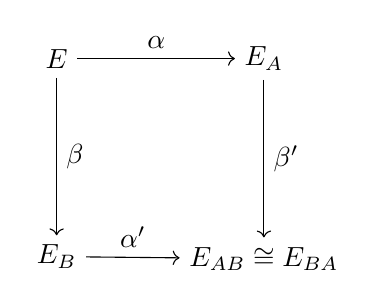
\begin{tikzpicture}[node distance = 2cm]
            \node (E) {$E$};
            \node (EA) [right = of E] {$E_A$};
            \node (EB) [below = of E] {$E_B$};
            \node (EAB) [below = of EA] {$E_{AB} \cong E_{BA}$};
            \draw [->] (E) -- node [above, midway] {$\alpha$} (EA);
            \draw [->] (E) -- node [right, midway] {$\beta$} (EB);
            \draw [->] (EA) -- node [right, midway] {$\beta'$} (EAB);
            \draw [->] (EB) -- node [above, midway] {$\alpha'$} (EAB);
        \end{tikzpicture}
    \end{center}
\end{proof}

\printbibliography

\end{document}